\documentclass[journal,12pt,twocolumn]{IEEEtran}
%\usepackage[left=1.5in,right=1in,top=1in,bottom=1in]{geometry}
%\usepackage[left=1.5in,right=1in]{geometry}
%\usepackage{geometry}
%\makeatletter%
%\textheight     243.5mm
%\textwidth      183.0mm
%\textwidth=31pc%
%\textheight=48pc
\usepackage{lipsum}% this package is included to get dummy paragraphs for sample purpose.
\usepackage{ulem}
\usepackage{alltt}
\usepackage{tfrupee}
\usepackage[anticlockwise,figuresright]{rotating}
\usepackage{pstricks}
\usepackage{wrapfig}
\usepackage{pstcol,pst-grad}
 \usepackage{bm}
\usepackage{enumitem}
\usepackage{listings}
    \usepackage{color}                                            %%
    \usepackage{array}                                            %%
    \usepackage{longtable}                                        %%
    \usepackage{calc}                                             %%
    \usepackage{multirow}                                         %%
    \usepackage{hhline}                                           %%
    \usepackage{ifthen}                                           %%
  %optionally (for landscape tables embedded in another document): %%
    \usepackage{lscape}     
    \usepackage{gensymb}     
    \usepackage{tabularx}
\usepackage{ifthen}%
\usepackage{amsmath}%
\usepackage{color}%
\usepackage{float}%	
\usepackage{graphicx}%
%\usepackage[right]{showlabels}%
\usepackage{boites}%
\usepackage{boites_exemples}%
\usepackage{graphicx,pstricks}
%\usepackage{enumerate}%
\usepackage{latexsym}
\usepackage[fleqn]{mathtools}
\usepackage{amssymb,amsfonts,amsthm}
\usepackage{mathrsfs,makeidx,listings,verbatim,moreverb}
%%\usepackage{amsthm,mathrsfs,makeidx,listings,verbatim,moreverb}
%\let\eqref\ref%  updated on 20th April 2017

\usepackage{hyperref}%
%\usepackage[dvips]{hyperref}%
\hypersetup{bookmarksopen=false}%
\usepackage{breakurl}%
\usepackage{tkz-euclide} % loads  TikZ and tkz-base

\newcommand{\solution}{\noindent \textbf{Solution: }}
\providecommand{\mbf}{\mathbf}
\providecommand{\rank}{\text{rank}}
\providecommand{\pr}[1]{\ensuremath{\Pr\left(#1\right)}}
\providecommand{\qfunc}[1]{\ensuremath{Q\left(#1\right)}}
\providecommand{\sbrak}[1]{\ensuremath{{}\left(#1\right)}}
\providecommand{\lsbrak}[1]{\ensuremath{{}\left(#1\right)}}
\providecommand{\rsbrak}[1]{\ensuremath{{}\left(#1\right)}}
\providecommand{\brak}[1]{\ensuremath{\left(#1\right)}}
\providecommand{\lbrak}[1]{\ensuremath{\left(#1\right.}}
\providecommand{\rbrak}[1]{\ensuremath{\left.#1\right)}}
\providecommand{\cbrak}[1]{\ensuremath{\left\{#1\right\}}}
\providecommand{\lcbrak}[1]{\ensuremath{\left\{#1\right.}}
\providecommand{\rcbrak}[1]{\ensuremath{\left.#1\right\}}}
\newenvironment{amatrix}[1]{%
  \left(\begin{array}{@{}*{#1}{c}|c@{}}
}{
	\end({array}\right)
}
\theoremstyle{remark}
\newtheorem{rem}{Remark}
\newtheorem{theorem}{Theorem}[section]
\newtheorem{problem}{Problem}
\newtheorem{proposition}{Proposition}[section]
\newtheorem{lemma}{Lemma}[section]
\newtheorem{corollary}[theorem]{Corollary}
\newtheorem{example}{Example}[section]
\newtheorem{definition}[problem]{Definition}
\newcommand{\sgn}{\mathop{\mathrm{sgn}}}
\providecommand{\abs}[1]{\left\vert#1\right\vert}
\providecommand{\res}[1]{\Res\displaylimits{#1}} 
\providecommand{\norm}[1]{\left\lVert#1\right\rVert}
%\providecommand{\norm}[1]{\lVert#1\rVert}
\providecommand{\mtx}[1]{\mathbf{#1}}
\providecommand{\mean}[1]{E\left[ #1 \right]}
\providecommand{\fourier}{\overset{\mathcal{F}}{ \rightleftharpoons}}
%\providecommand{\hilbert}{\overset{\mathcal{H}}{ \rightleftharpoons}}
\providecommand{\system}{\overset{\mathcal{H}}{ \longleftrightarrow}}
	%\newcommand{\solution}[2]{\textbf{Solution:}{#1}}
%\newcommand{\solution}{\noindent \textbf{Solution: }}
\newcommand{\cosec}{\,\text{cosec}\,}
\providecommand{\dec}[2]{\ensuremath{\overset{#1}{\underset{#2}{\gtrless}}}}
\newcommand{\myvec}[1]{\ensuremath{\begin{pmatrix}#1\end{pmatrix}}}
\newcommand{\myaugvec}[2]{\ensuremath{\begin{amatrix}{#1}#2\end{amatrix}}}
\newcommand{\mydet}[1]{\ensuremath{\begin{vmatrix}#1\end{vmatrix}}}
\newcommand\figref{Fig.~\ref}
\newcommand\appref{Appendix~\ref}
\newcommand\tabref{Table~\ref}
\newcommand{\romanNumeral}[1]{\uppercase\expandafter{\romannumeral#1}}
%\numberwithin{equation}{section}
%\numberwithin{equation}{subsection}
%\numberwithin{problem}{section}
%\numberwithin{definition}{section}
%\makeatletter
%\@addtoreset{figure}{problem}
%\makeatother

%\let\StandardTheFigure\thefigure
\let\vec\mathbf
\def\inputGnumericTable{}                                 %%
%New macro definitions
\newcounter{matchleft}\newcounter{matchright}

\newenvironment{matchtabular}{%
  \setcounter{matchleft}{0}%
  \setcounter{matchright}{0}%
  \tabularx{\textwidth}{%
    >{\leavevmode\hbox to 1.5em{\stepcounter{matchleft}\arabic{matchleft}.}}X%
    >{\leavevmode\hbox to 1.5em{\stepcounter{matchright}\alph{matchright})}}X%
    }%
}{\endtabularx}


\renewcommand\thesection{\arabic{section}}
\renewcommand\thesubsection{\thesection.\arabic{subsection}}
\renewcommand\thesubsubsection{\thesubsection.\arabic{subsubsection}}

\renewcommand\thesectiondis{\arabic{section}}
\renewcommand\thesubsectiondis{\thesectiondis.\arabic{subsection}}
\renewcommand\thesubsubsectiondis{\thesubsectiondis.\arabic{subsubsection}}

\extrafloats{200}

\bibliographystyle{IEEEtran}


\def\BibTeX{{\rm B\kern-.05em{\sc i\kern-.025em b}\kern-.08em
    T\kern-.1667em\lower.7ex\hbox{E}\kern-.125emX}}
\title{
\vspace{1cm}

\includegraphics[width=0.15\textwidth]{1.jpg} \\ Seven Segment Assignment} 
\author{T AKHILA\\ Roll No: FWC22312 \\ akhilathalla0104@gmail.com}


\begin{document}
\maketitle
\section{Abstract}
This paper presents the design and implementation of a 7-segment display control system using an Arduino Uno and programmed via Termux, a Linux terminal emulator for Android devices. The system provides a portable, cost-effective solution for controlling numerical displays without the need for a traditional desktop environment.

This paper details the hardware setup, the programming of the display using the Arduino, and the configuration of Termux for seamless coding and uploading. This approach offers a practical solution for enthusiasts and students, facilitating mobile development of embedded systems.

\section{Components}
\begin{tabularx}{0.46\textwidth} { 
  | >{\centering\arraybackslash}X 
  | >{\centering\arraybackslash}X 
  | >{\centering\arraybackslash}X
  | >{\centering\arraybackslash}X | }
\hline
\textbf{Component}& \textbf{Values} & \textbf{Quantity}\\
\hline
Arduino & UNO & 1 \\  
\hline
JumperWires & M-F & 30 \\ 
\hline
seven segment &common Anode &1\\
\hline
Bread-board & & 1\\
\hline
Resistors &220ohms &1\\

\hline
\end{tabularx}

 \begin{center}
Table.Components
 \end{center}

 \section{Pin Diagram}




\begin{center}

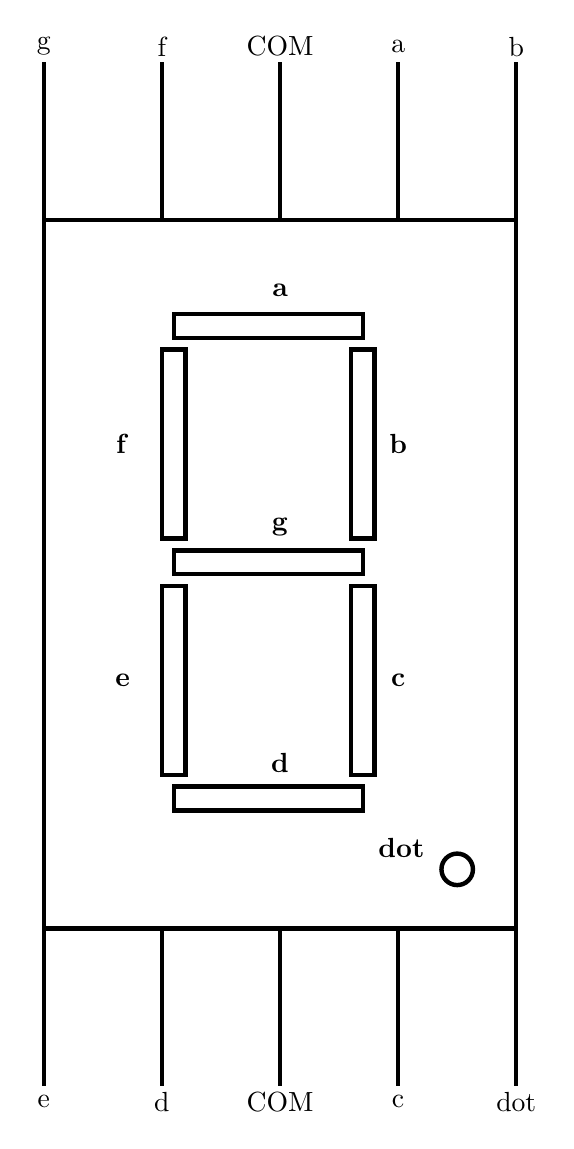
\begin{tikzpicture}
  [
    scale=1,
    >=stealth,
    point/.style = {draw, circle,  fill = black, inner sep = 0.5pt},
    dot/.style   = {draw, circle,  fill = black, inner sep = .2pt},
  ]

%Vertices of the main display rectangle
\def \xmin{0}
\def \xmax{6}
\def \ymin{0}
\def \ymax{-9}

%Number of pins on a side
\def \n{5}
\def \k{1.6}

%Draw the display rectangle
\draw[ultra thick] (\xmin,\ymin)rectangle (\xmax,\ymax);

%Define height of pins and their separation
\def \height{2}
\pgfmathsetmacro{\wid}{(\xmax-\xmin)/(\n-1)}

%Defining y axis divisions
\pgfmathsetmacro{\ywid}{(\ymin-\ymax)/(\n-2)}

\foreach \i in {0,...,4}
{
\draw[ultra thick] (\xmin + \i*\wid, \ymin) -- (\xmin + \i*\wid, \ymin + \height); 
\draw[ultra thick] (\xmin + \i*\wid, \ymax) -- (\xmin + \i*\wid, \ymax -\height); 
}
%%
%%%
\foreach [count=\i] \j in {g,f,COM,a,b}{
            \node (\i) at ( -1.5 + \i*\wid,\height+0.2) {\j} ;
            }
\foreach [count=\i] \j in {e,d,COM,c,dot}{
            \node (\i) at ( -1.5 + \i*\wid,\ymax -\height-0.2) {\j} ;
            }

\foreach [count=\i] \j in {\textbf{a},\textbf{g},\textbf{d}}
{            
\draw[ultra thick] (\xmin+1.1*\wid,{\ymin-(\i-0.5)*\ywid} ) rectangle +(\k*\wid,0.3 );
\node (\i) at ( \xmin + 2*\wid,{\ymin-(\i-0.7)*\ywid}) {\j} ;
}
\foreach [count=\i] \j in {\textbf{f},\textbf{e}}
{            
\draw[ultra thick] (\xmin+\wid,{\ymin-(\i+0.35)*\ywid} ) rectangle +(0.3,\k*\wid );
\node (\i) at ( \xmin + \wid-0.5,{\ymin-(\i-0.05)*\ywid}) {\j} ;
}
\foreach [count=\i] \j in {\textbf{b},\textbf{c}}
{            
\draw[ultra thick] (\xmin+2.6*\wid,{\ymin-(\i+0.35)*\ywid } ) rectangle +(0.3,\k*\wid );
\node (\i) at ( \xmin + 3*\wid,{\ymin-(\i-0.05)*\ywid}) {\j} ;
}


%
\draw[ultra thick] (\xmax - 0.5*\wid,{\ymax+0.25*\ywid}) circle [radius=0.2];
\draw[ultra thick](\xmax - 0.5*\wid,{\ymax+0.25*\ywid}) node[sloped, anchor=center, above, text width=2.0cm]{\textbf{dot}};    
\end{tikzpicture}
\end{center}


\section{Proceduer}
\begin{enumerate}
    \item Make the connections between Arduino and Seven Segment as per the below Table


\begin{table}[h!]
    \centering
    \small  % This makes the font size smaller for the table content
    \begin{tabular}{|c|c|c|c|c|c|c|c|}
        \hline
        \textbf{Arduino}  & 2 & 3 & 4 & 5 & 6 & 7 & 8\\
        \hline
        \textbf{Display} &a&b&c&d&e&f&g\\
        \hline
    \end{tabular}\\
     \begin{center} 
 Table.Connections
 \end{center}
\end{table} 
    \item Download code from the below source and execute using Arduino droid \\

    \begin{tabularx}{0.46\textwidth} { 
  | >{\centering\arraybackslash}X |}
  \hline
   https://github.com/Akhilathalla/Akhila/blob/main/Sevensegment/main.cpp\\
  \hline
\end{tabularx}
 
\end{enumerate}


\section{Result}
\begin{figure}[h] 
	\centering 
	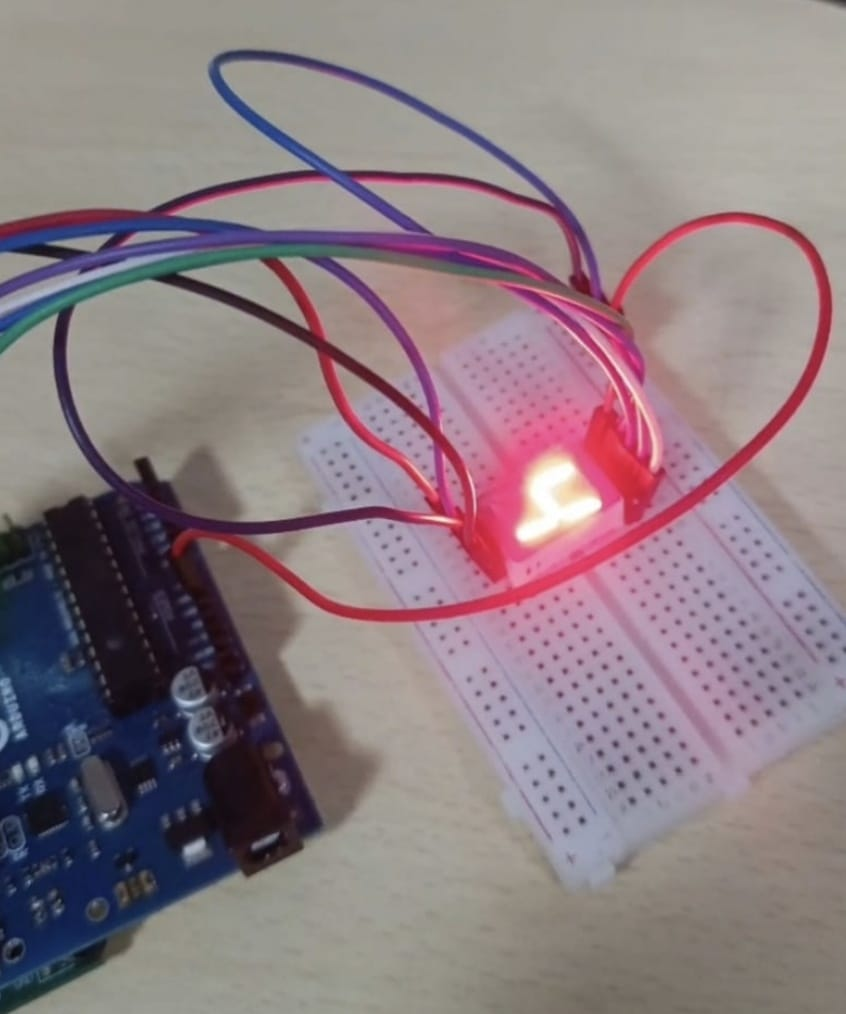
\includegraphics[width=0.4\textwidth]{2.jpg}
\centering	
\caption{\label{fig:Gate}}    
\end{figure}

\section{Conclusion}
Hence implementation of Seven segment dispaly using arduino is done.
\end{document}
